\documentclass{article}

\usepackage[utf8]{inputenc}
\usepackage{parskip}
\usepackage{graphicx}
\usepackage{epstopdf}
\usepackage{wrapfig}
\usepackage{mwe}
\usepackage{libertine}
\usepackage{inconsolata}
\usepackage{hyperref}

\newcommand\theversion{0.0.1-git}

\hypersetup{
  hidelinks,
  pdftitle={Pancakes v\theversion},
  pdfauthor={Johann Tutor}
}

\renewcommand{\sectionautorefname}{§}
\renewcommand{\subsectionautorefname}{§}
\renewcommand{\subsubsectionautorefname}{§}
\renewcommand{\paragraphautorefname}{¶}

\setcounter{secnumdepth}{4}

\begin{document}
\title{Pancakes\\ \large A flipping card game, v\theversion}
\author{Johann Tutor}
\date{\today}
\maketitle

Pancakes is a quick and easy-to-learn card game developed by Johann Tutor.

When teaching this game to a friend, it is recommended that they play without being told the rules for the first game;
only answer ``yes''/``no'' questions and correct them when they do something illegal.

\tableofcontents

\newpage

\section{Requirements}

Pancakes uses a standard deck of cards with Jokers.
Up to five players may play.

\section{Setting Up}
\label{sec:setup}

Shuffle the deck. Deal eight cards face-down on the table, then deal one card face-up on each of those to form eight Stacks.
These Stacks should be arranged in four centered rows with 1-3-3-1 Stacks each.

Deal five cards to each player and set aside the rest of the deck to be the Draw Pile. Decide on a player order.

\section{Rules}

On each turn, you must place a card of the same number on to one of the Stacks; this is a ``legal play''. You may do so in one of two ways: put down a card from your hand, or transfer a card from one Stack to another. If you cannot make a legal play, you must pass. You may only play one card per turn.

\subsection{Playing a Card}
\label{sec:playcard}

A card may only be placed on an empty Stack or on a Stack whose top card is either the same number, a Joker or a card back.

If the card you play is a different color than the one on the top of the Stack, flip the Stack so that the card on the bottom is now on top.

Empty Stacks and card backs are always considered the same color as the card put on top unless the card is a Joker.
In other words, placing a card that is not a Joker on top of an empty Stack or a card back does not flip the Stack.

Jokers are always considered a different color than the card on which it is placed or the card that is put on top of it, including empty Stacks and card backs.
In other words, playing a Joker or playing any card on top of a Joker flips the Stack, even if it is the only card in the Stack.

\subsubsection{Playing From Your Hand}
\label{sec:fromhand}

On your turn, you may choose to play from your hand.

\paragraph{}
If you have a card that you may legally play, play it.

\paragraph{}
If you do not have any cards that you may legally play, draw from the Draw Pile until you draw a card that you may legally play, then play that card.

\paragraph{}
You cannot draw if you have any legal plays in your hand and you must play the first card that gives you a legal play when drawing.
However, if you accidentally started drawing illegally (i.e. you had a legal play in your hand), you must continue to draw until you draw a card that you may legally play. Any cards that would have been legal to play cannot be played until your next turn.

\paragraph{}
If the Draw Pile is or becomes empty while drawing, you must pass as you have no legal plays.

\paragraph{}
You may not play from a Stack until your next turn once you have started drawing.

\paragraph{}
If you have no more cards in your hand at the end of your turn, the game ends immediately.

\subsubsection{Playing From a Stack}
\label{sec:fromstack}

On your turn, you may choose to play from a Stack instead of your hand. Note that if you have already started drawing, you may not play from a Stack until your next turn.

\paragraph{}
Provided it is a legal play, take the top card of one Stack and place it on the other Stack. Flip if necessary.

\paragraph{}
If you expose a card back on the first Stack, flip the top card (not the Stack) so that it is face-up.

\subsection{Passing}

You may only pass if you have no legal plays.

If everyone passes in succession, shout ``Pancakes!'' and flip all Stacks. If everyone passes immediately after that, the game ends.

\subsection{Winning}

The player who empties their hand first wins the game. If the game ends with everyone passing, the player with the least number of cards in their hand wins the game; if there are multiple players with the least number of cards, they tie.

\section{Scoring}

Points go to the winner of the game. The winner's score is calculated as follows: count the number of cards that the other players have, subtract the number of cards the winner has, divide that by one less than the number of players, and round up to the nearest whole number.

For the mathematically inclined:

$$
\langle\textrm{Score}\rangle = \left\lceil\frac{\langle\textrm{others'\ cards}\rangle - \langle\textrm{winner's\ cards}\rangle}{\langle\textrm{\#\ of\ players} - 1\rangle}\right\rceil
$$

\section{Glossary}
\begin{description}
  \item[Stack] (\autoref{sec:setup})\\
    An area where a card may be played.
\end{description}

\medskip
\hrule

{
  \small
  \includegraphics[scale=0.5]{cc-by.eps}\\
  This work is licensed under the Creative Commons Attribution 4.0
  International License. To view a copy of this license, visit
  \url{http://creativecommons.org/licenses/by/4.0/} or send a letter to Creative Commons, PO Box 1866, Mountain View, CA 94042, USA.
}

\end{document}
